\section{Methodology}

This work consists of three parts, data generation, hyperparameter search,
model training, and prediction. To generate
data needed for training our \ model we used the \texttt{TrainARMA}
functionality
in the \texttt{RAVEN} tool from INL to generate synthetic histories. These
scenarios are passed to the \acrshort{ESN} model for training and testing.
The \acrshort{ESN} is implemented with the open-source code \texttt{pyESN}
\cite{korndorfer_pyesn_2015}.
\subsection{Scenario Generation}
In this work we use the scenario generation method described in Baker et. al
using the \texttt{RAVEN} framework \cite{baker_optimal_2018}. The algorithm for
producing synthetic histories is:
\begin{enumerate}
	\item Create a ``typical year`` from historical data.
	\item Fit an Autoregressive Moving Average (ARMA) model using
	\texttt{TrainARMA}.
	\item Use Monte Carlo sampling to generate synthetic histories from ARMA
	 model.
\end{enumerate}

We perform this process for three datasets: Electricity demand, wind generation,
and solar generation. This allows us to train an \acrshort{ESN} model to
predict generation
from wind and solar farms and to predict the net demand profile given by
\begin{equation}
	\label{eqn:net-demand}
	\begin{split}
		D_{net} & = (D_{total} - P_{wind} - P_{pv})_h \text{ $\forall$ $h$ in }
		[0,8759]
	\end{split}
\end{equation}

Where $D_{total}$ is the total demand at a given hour, $h$, of a synthetic
demand profile from the
ARMA model.

\subsection{Reservoir Computing Model}

Unlike a typical feed forward neural network, an ``echo state network'' (also
called a ``liquid state machine'') is a type of
recurrent neural network that uses a single layer of many neurons called a
``reservoir''. The reservoir has an adjacency matrix $\bm{A}$ that is
\begin{enumerate}
	\item sparsely populated
	\item connected by uniformly random weights centered at zero
	\item has a large number of neurons
\end{enumerate}
A reservoir computer also satisfies the \textit{echo state property}
\cite{pathak_model-free_2018, lukosevicius_reservoir_2009}. This
property ensures that a system's state has a decaying influence on future states
(like an echo of sound or ripples on water). This property is satisfied in most
cases when the spectral radius (the absolute value of the greatest eigenvalue of
$\bm{A}$)\cite{lukosevicius_reservoir_2009} is,
\begin{align}
	\rho(\bm{A}) < 1.
\end{align}
However, the echo state property can still be satisfied for a spectral radius
greater than unity \cite{lukosevicius_practical_2012}.

\begin{figure}[H]
	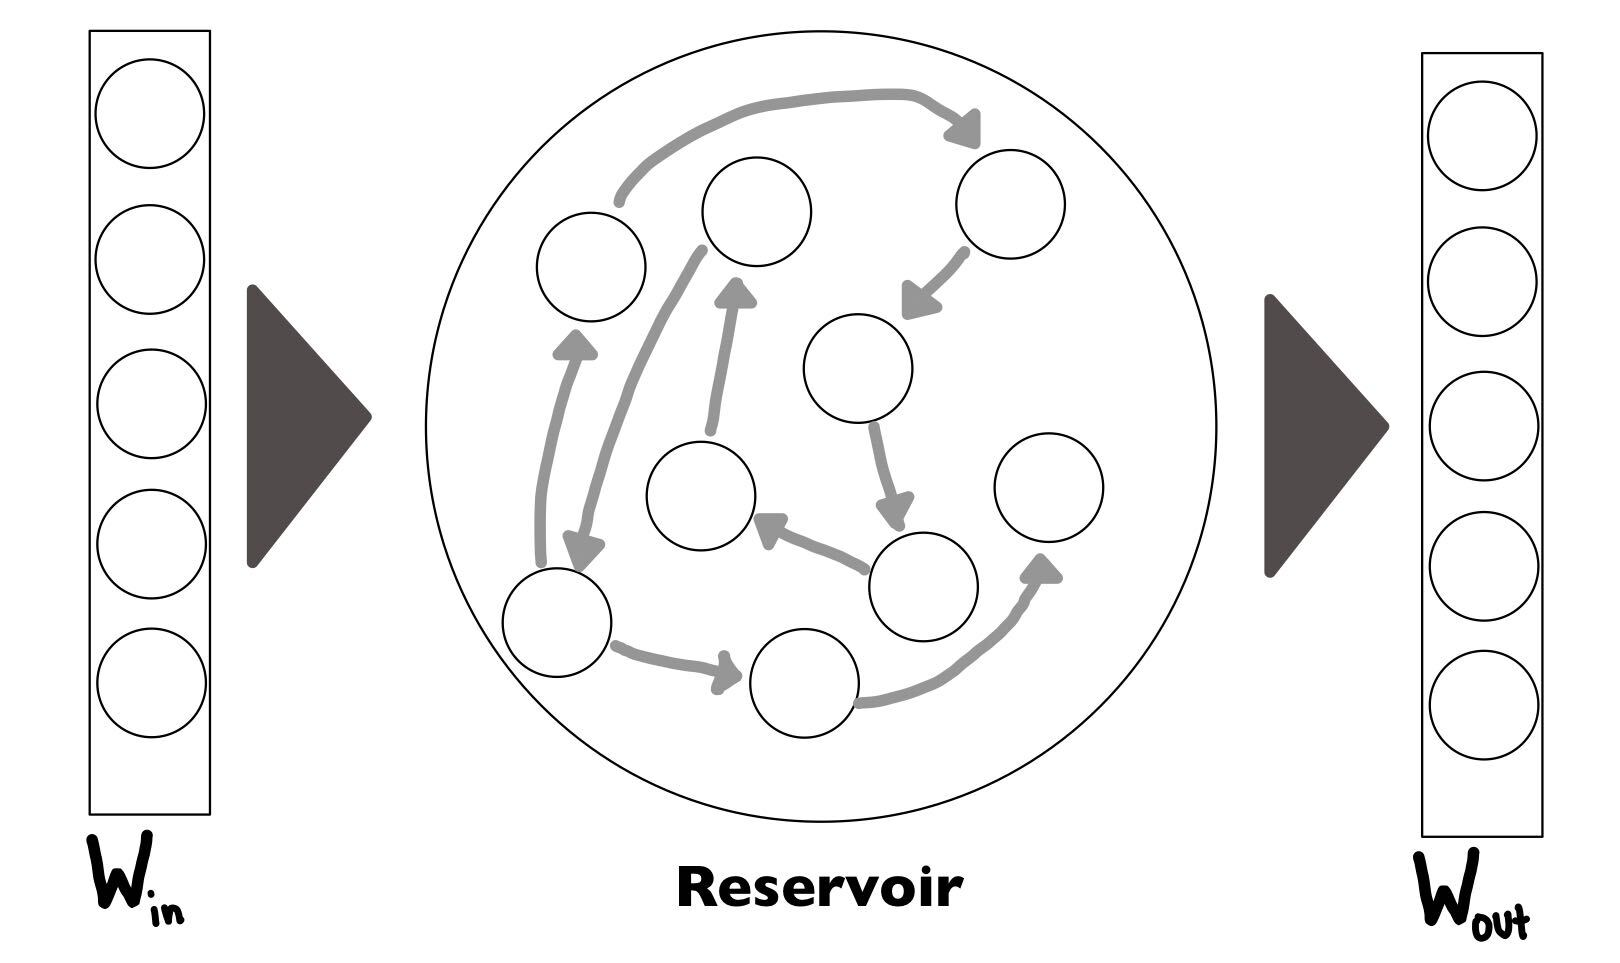
\includegraphics[width=\columnwidth]{reservoir_network.jpg}
	\caption{A basic reservoir computer or echo state network.The connections in
	the reservoir are given by $\bm{A}$}
	\label{fig:RCmodel}
\end{figure}

Figure \ref{fig:RCmodel} gives an visual representation of a basic
\acrshort{ESN}. An
input vector of length \textit{K} is mapped to the reservoir layer by an input
weight matrix $\bm{W_{in}}$. The state of the reservoir is mapped to an output
layer of length \textit{N} with an output weight matrix $\bm{W_{out}}$. In this
work, the input vector is a function of time, $\bm{u}(t)$, and the output
vector is the next state of the system, $\bm{u}_p(t+\Delta t)$. Ideally, the
difference between the prediction, $\bm{u}_p$, and the actual, $\bm{u}_a$, is
minimized. During training, the output weight matrix is trained through
backpropagation using a loss function like cross entropy
\cite{pathak_model-free_2018, vlachas_backpropagation_2020}.

\subsection{Hyperparameter Search}
Due to the architecture of \acrshort{ESN}s the weights and connections
inside the reservoir do not need to be trained and, in our choice of
implementation, cannot be. This dramatically reduces the training time because
only the linear output layer needs to be trained. One drawback of this approach
is its sensitivity to hyperparameters, which must be carefully chosen before
running the network. Here, we perform grid searches over a variety of networks
to establish which combination of hyperparameters minimizes the mean squared
error of the model,
\begin{align}
	MSE &= \frac{1}{N}\sum_i^N (\hat{y} - y_i)^2\\
	\intertext{where}
	\hat{y} &= \mbox{the average value of the ouput.}\nonumber
\end{align}
